\documentclass[a4paper,10pt]{article}
\usepackage{graphicx}
\usepackage{float}
\usepackage{booktabs}
\usepackage{amsmath,amssymb,amsthm}
\usepackage{physics}
\usepackage{mathtools}
\usepackage{geometry}
\geometry{a4paper,tmargin=4cm,bmargin=3.5cm, lmargin=3cm,rmargin=3cm}

\title{Caratterizzazione rivelatore a barriera superficiale}
\author{Gianluca Cavallaro \\ Marco Gobbo}
\date{24 Marzo 2020}
\begin{document}
\maketitle

%%% INTRODUZIONE %%%

\section{Introduzione}
    L'obiettivo di questa parte dell'esperienza \`e quello di allestire, ottimizzare e caratterizzare il rivelatore che verr\`a in seguito utilizzato per lo studio dell'interazione delle particelle alfa con la materia. In questo report ci proponiamo di analizzare le misurazioni acquisite, effettuandone l'analisi.

%%% STRUMENTAZIONE %%%

\section{Strumentazione}
\begin{itemize}
    \item Crate NIM per alimentazione di moduli di elettronica standard
    \item Modulo 7401-7401VR Alpha Spectrometer CANBERRA
    \item Scheda ACD/MCA CAEN N957
    \item PC di controllo per la scheda ACD/MCA
    \item Pompa rotativa e circuito per l'evacuazione della camera
    \item Rivelatori di Silicio a barriera superficiale (900 mm\textsuperscript{2} di area)
    \item Sorgente alpha di 241-Am
\end{itemize}

%%% CARATTERIZZAZIONE CON PULSER %%%

\section{Caratterizzazione con impulsatore calibrato in energia}
Dopo aver posto il rivelatore al Silicio in una camera a vuoto, si sfutta la catena di lettura classica (pre-amplificatore, amplificatore, shaper, ACD/MCA) per generare sull'elettronica in uscita dei segnali la cui forma \`e analoga a quella che il rivelatore fornisce in seguito ad una interazione alfa. Come indicato, nel caso specifico il rivelatore \`e polarizzato con una tensione di 50 V. Si fissano dei precisi valori di energia dell'impulsatore, in un intervallo che va da 1 MeV a 10 MeV, e con i dati ottenuti si costruiscono diversi istogrammi, uno per ciascun valore di energia. Da ognuno di questi istogrammi, tramite una estrapolazione gaussiana, \`e possibile ricavare la posizione, espressa in mV, del picco. Di seguito sono riportate le posizioni dei 10 picchi, relative alle 10 raccolte dati a nostra disposizione:
\begin{center}
    \begin{tabular}{ccc}
        \toprule
        Energia [MeV] & Tensione picco [mV] & $\sigma$ [mV]\\
        \midrule
        1.10 & 665 & 7\\
        2.09 & 1424 & 7\\
        3.09 & 2184 & 7\\
        4.09 & 2944 & 7\\
        5.09 & 3707 & 8\\
        6.09 & 4468 & 8\\
        7.09 & 5227 & 8\\
        8.09 & 5983 & 8\\
        9.09 & 6734 & 8\\
        9.98 & 7405 & 8\\
        %1.10 & 665 & 7.76\\
        %2.09 & 1424 & 7.85\\
        %3.09 & 2184 & 7.88\\
        %4.09 & 2944 & 7.74\\
        %5.09 & 3707 & 7.70\\
        %6.09 & 4468 & 7.79\\
        %7.09 & 5227 & 7.76\\
        %8.09 & 5983 & 7.75\\
        %9.09 & 6734 & 7.75\\
        %9.98 & 7405 & 7.74\\
        \bottomrule
    \end{tabular}\\
\end{center}

\noindent Attraverso questi dati, si va a costruire un grafico \textit{energia vs tensione picco}. Questo grafico rappresenta la \textbf{curva di calibrazione}:

\begin{figure}[h!]
    \centering
    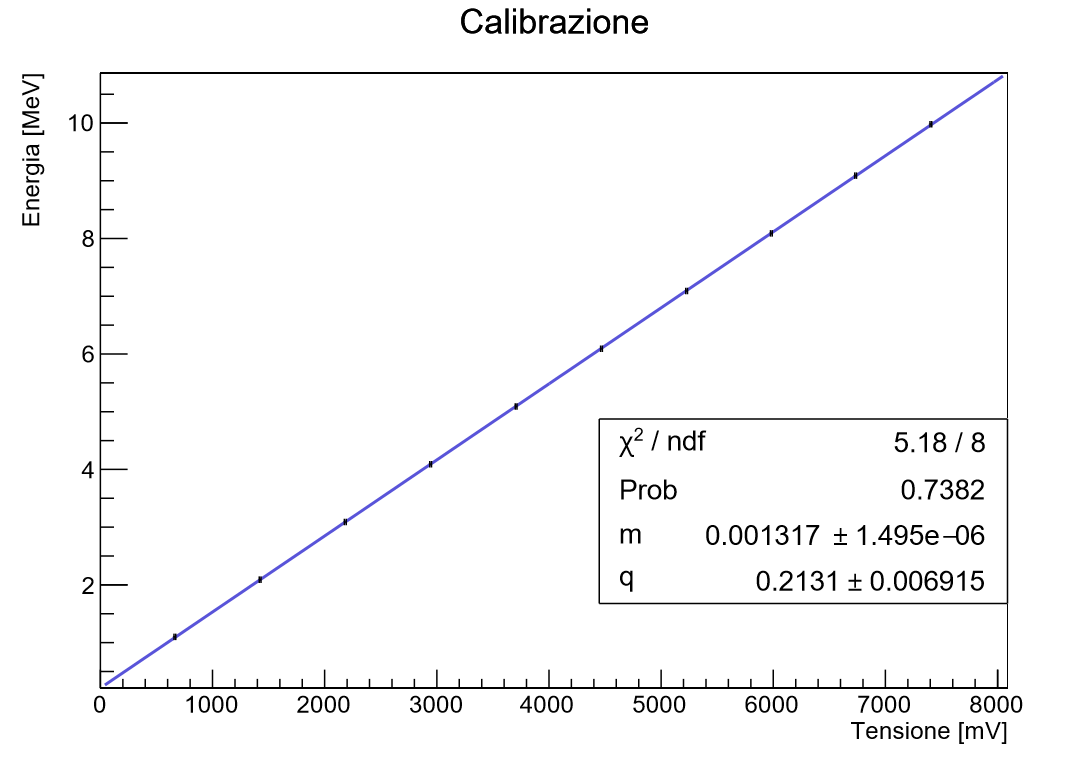
\includegraphics[scale=0.7]{rettacalibrazione.jpg}
    \caption{Retta di calibrazione Energia vs Tensione Picco}
\end{figure}

\noindent Dal fit, si ottiene la seguente retta di calibrazione:
$$
    Energia = m \cdot Picco + q
$$
Con coefficienti pari a:
$$
    m = 1.327\cdot10^{-3} \pm 10^{-6}\, \frac{MeV}{mV}
$$
$$
    q = 0.213 \pm 0.7\cdot10^{-2}\, MeV
$$

\noindent Con i seguenti valori per quanto riguarda $\chi$\textsuperscript{2} ridotto e \textit{P-Value}:
$$
    \frac{\chi\textsuperscript{2}}{NDF} = \frac{5.18}{8} = 0.6475
$$
$$
    \textit{P-Value} = 0.7382
$$
%% OSSERVAZIONI %%

\subsection{Osservazioni}
Il grafico di calibrazione ottenuto mostra con chiarezza l'andamento lineare della relazione fra energia e tensione del picco. Si pu\`o notare che l'intercetta della retta infatti \`e prossima all'origine: questa piccola discrepanza pu\`o essere dovuta ad un offset di base dello strumento. 
\`E necessario per\`o verificare l'attendibilit\`a dei risultati ottenuti andando a confrontare con lo spettro di una sorgente nota.

%% SORGENTE 241-Am %%

\section{Caratterizzazione con sorgente di 241-Am}
In questa parte successiva, nella camera viene inserita una sorgente di 241-Am, e ci\`o che in questo caso viene misurato \`e lo spettro in energia di questo materiale. Di seguito \`e riportato lo spettro della sorgente:

\begin{figure}[h!]
    \centering
    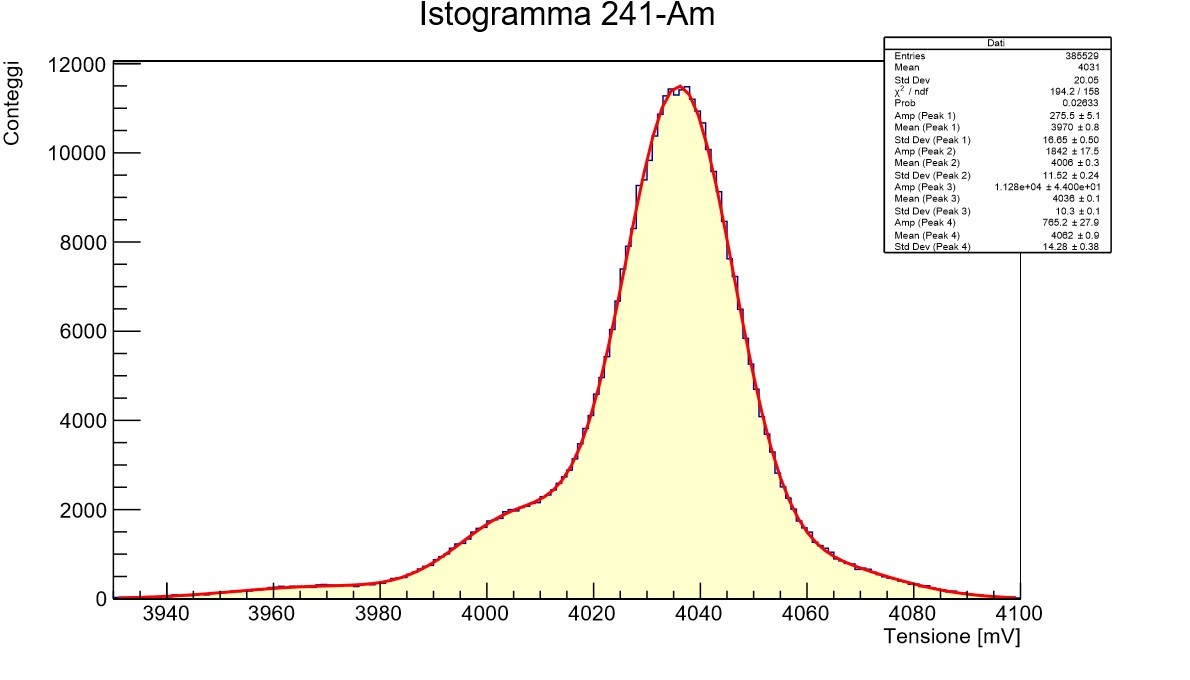
\includegraphics[scale=0.7]{istoame.jpg}
    \caption{Spettro 241-Am}
\end{figure}

\noindent Con i seguenti valori per quanto riguarda $\chi$\textsuperscript{2} ridotto e \textit{P-Value}:
$$
    \frac{\chi\textsuperscript{2}}{NDF} = \frac{194.2}{158} = 1.229
$$
$$
    \textit{P-Value} = 0.0263
$$

\noindent Ed i seguenti valori per ciascun picco:

\begin{center}
    \begin{tabular}{cc}
        \toprule
        Picco Canale[mV] & $\sigma$[mV] \\
        \midrule
        3970 & 17\\
        4006 & 12\\
        4036 & 10\\
        4062 & 14\\
        \bottomrule
    \end{tabular}\\
\end{center}

\noindent Dal fit \`e possibile dunque risalire ai 4 picchi di emissione del 241-Am. Utilizzando le energie di emissione tabulate, si costruisce una nuova curva di calibrazione:

\begin{figure}[H]
    \centering
    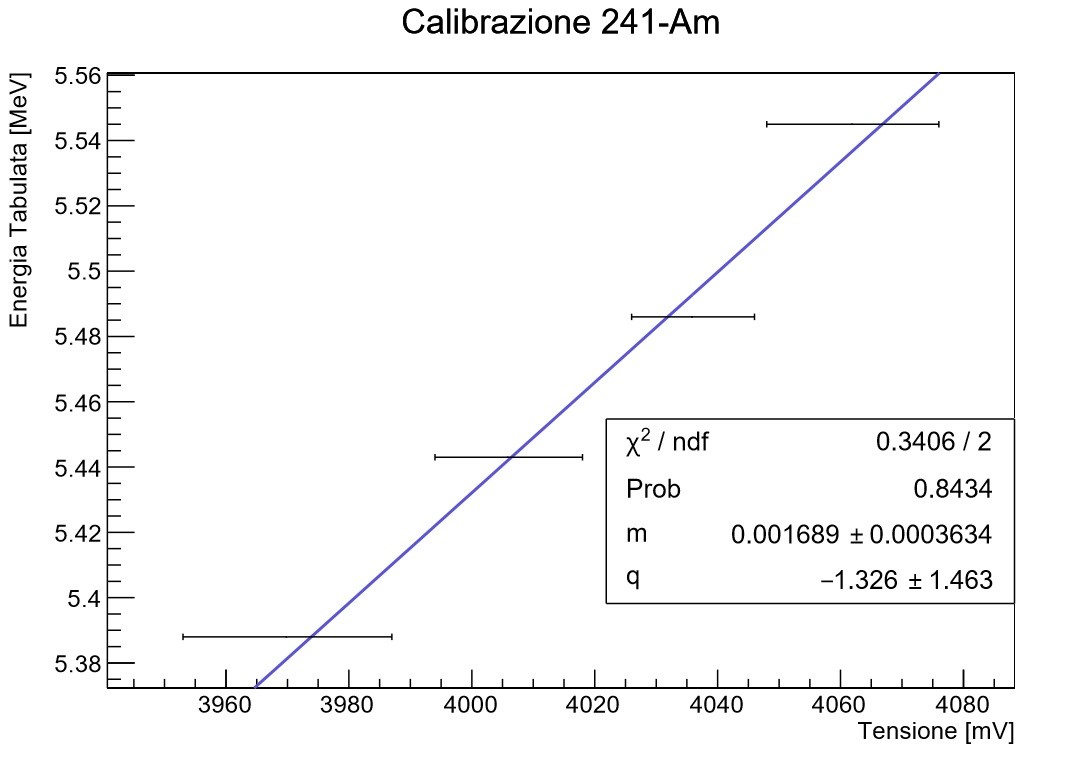
\includegraphics[scale=0.7]{rettaame.jpg}
    \caption{Retta di calibrazione per il 241-Am}
\end{figure}
$$
    Energia = m \cdot Picco + q
$$
Con coefficienti pari a:
$$
    m = 1.7\cdot10^{-3} \pm 3.6\cdot10^{-4}\, \frac{MeV}{mV}
$$
$$
    q = - 1.3 \pm 1.5\, MeV
$$

\noindent Con i seguenti valori per quanto riguarda $\chi$\textsuperscript{2} ridotto e \textit{P-Value}:
$$
    \frac{\chi\textsuperscript{2}}{NDF} = \frac{0.3406}{2} = 0.1703
$$
$$
    \textit{P-Value} = 0.8434
$$

\noindent Di seguito viene invece riportata la tabella che mostra il confronto fra l'energia tabulata del 241-Am e l'energia calcolata tramite da retta di calibrazione ottenuta al primo punto:

\begin{center}
    \begin{tabular}{ccccc}
        \toprule
        Canale & E [keV] & $\sigma$ [keV] & Energia tabulata[keV] & Compatibilit\`a \\
        \midrule
        3970 & 5441.59 & 23.76 & 5388 & 2.41\%\\
        4006 & 5489.00 & 17.70 & 5443 & 0.93\%\\
        4036 & 5528.51 & 15.40 & 5486 & 0.58\%\\
        4062 & 5562.75 & 20.15 & 5545 & 37.71\%\\
        \bottomrule
    \end{tabular}\\
\end{center}

\noindent Al fine confrontare la compatibilit\`a tra i valori tabulati e i valori ricavati dalla retta di calibrazione, si assume che la distribuzione di ogni singolo picco sia gaussiana.\\
Per questo motivo si effettua un test di compatibilit\`a di tipo gaussiano con significativit\`a del 5\%.
Si calcola il valore assoluto $\tau$ dello scarto normalizzato tra il valore tabulato e il valore calcolato:
$$
    \tau = \abs\Big{\frac{E_t - E_c}{\sigma_{E_c}}}
$$
E si valuta quest'ultimo utilizzando il complementare della funzione degli errori:
$$
    Erfc(\tau) = \frac{2}{\sqrt{\pi}}\int_{\tau}^{+\infty} e^{-x^2}\, dx
$$

\noindent Come ultima cosa, \`e nostro interesse calcolare la risoluzione del rivelatore. Sfruttando la relazione

$$
    R=\frac{FWHM}{Picco[mV]}
$$
andiamo a calcolare quella che \`e la risoluzione relativa per ognuno dei picchi estrapolati. La risoluzione relativa viene poi moltiplicata per l'energia corrispondente del picco, in modo da ottenere la risoluzione energetica. Si ottengono i seguenti risultati:

\begin{center}
    \begin{tabular}{cccc}
        \toprule
        Canale[mV] & Risoluzione relativa & Energia [keV] & Risoluzione energetica [keV] \\
        \midrule
        3970 & 0.01 & 5441.59 & 54.7\\
        4006 & 0.007 & 5489.00 & 38.6\\
        4036 & 0.005 & 5528.51 & 32.2\\
        4062 & 0.008 & 5562.75 & 45.1\\
        \bottomrule
    \end{tabular}\\
\end{center}

\noindent Andiamo a mostrare l$'$andamento della risoluzione energetica in funzione dei picchi stessi:

\begin{figure}[H]
    \centering
    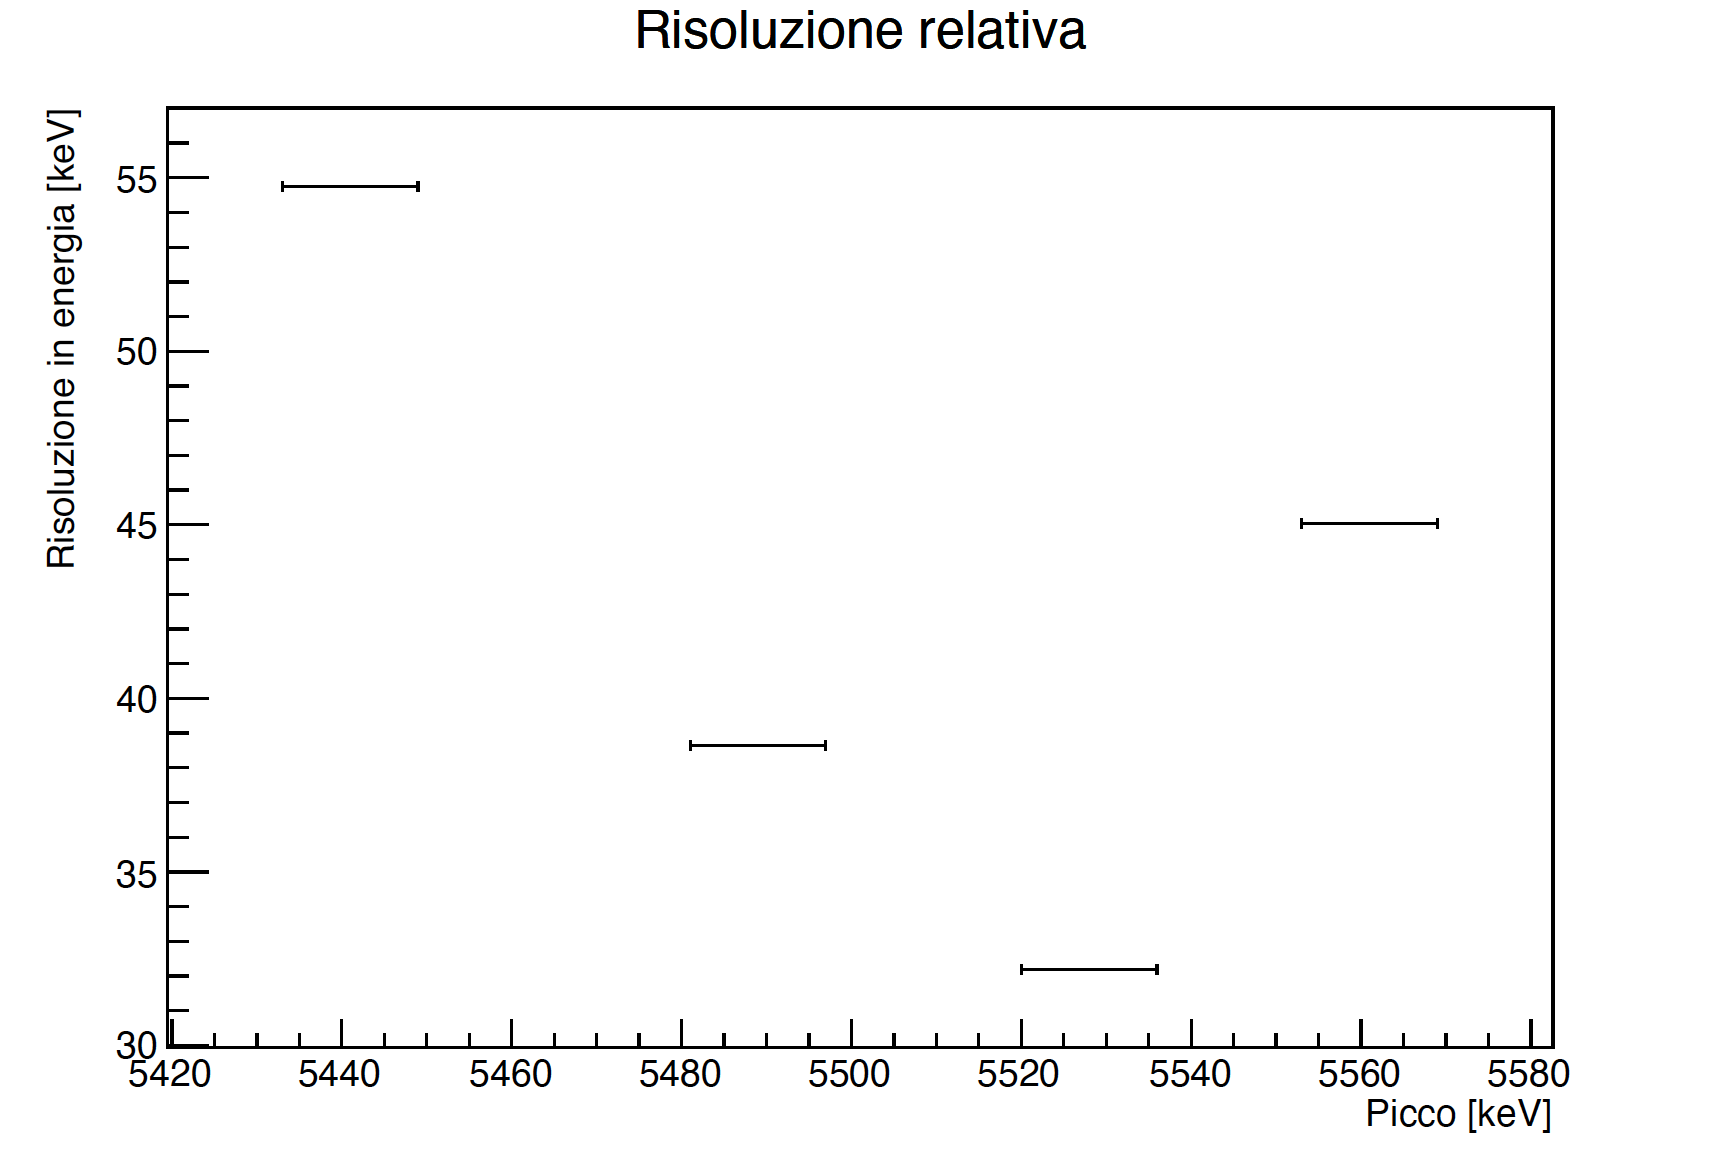
\includegraphics[scale=0.4]{risoluzione.png}
    \caption{Risoluzione energetica in funzione del picco di energia}
\end{figure}

%% OSSERVAZIONI %%

\subsection{Osservazioni}
I dati che abbiamo elaborato mostrano alcune informazioni importanti. I test di compatiblit\`a mettono in evidenza che soltanto il quarto picco \`e compatibile con il valore tabulato mentre i primi tre hanno una discrepanza intorno ai 40 keV. Si potrebbe supporre dunque che questa differenza sia collegata ad un offset interno a tutta la catena di lettura. Andando a rappresentare un grafico della discrepanza in funzione dell'energia calcolata (Figura 5) si pu\`o constatare che questo ipotetico offset sia costante per tutti e tre i valori tranne ovviamente per il quarto picco. Questo non deve assolutamente preoccuparci poich\'e si tratta di un picco a bassa statistica (analizzando la Figura 2, il quarto picco a 4062 mV non \`e nemmeno osservabile) e dunque risulta complicato andarne a valutare i parametri.

\begin{figure}[H]
    \centering
    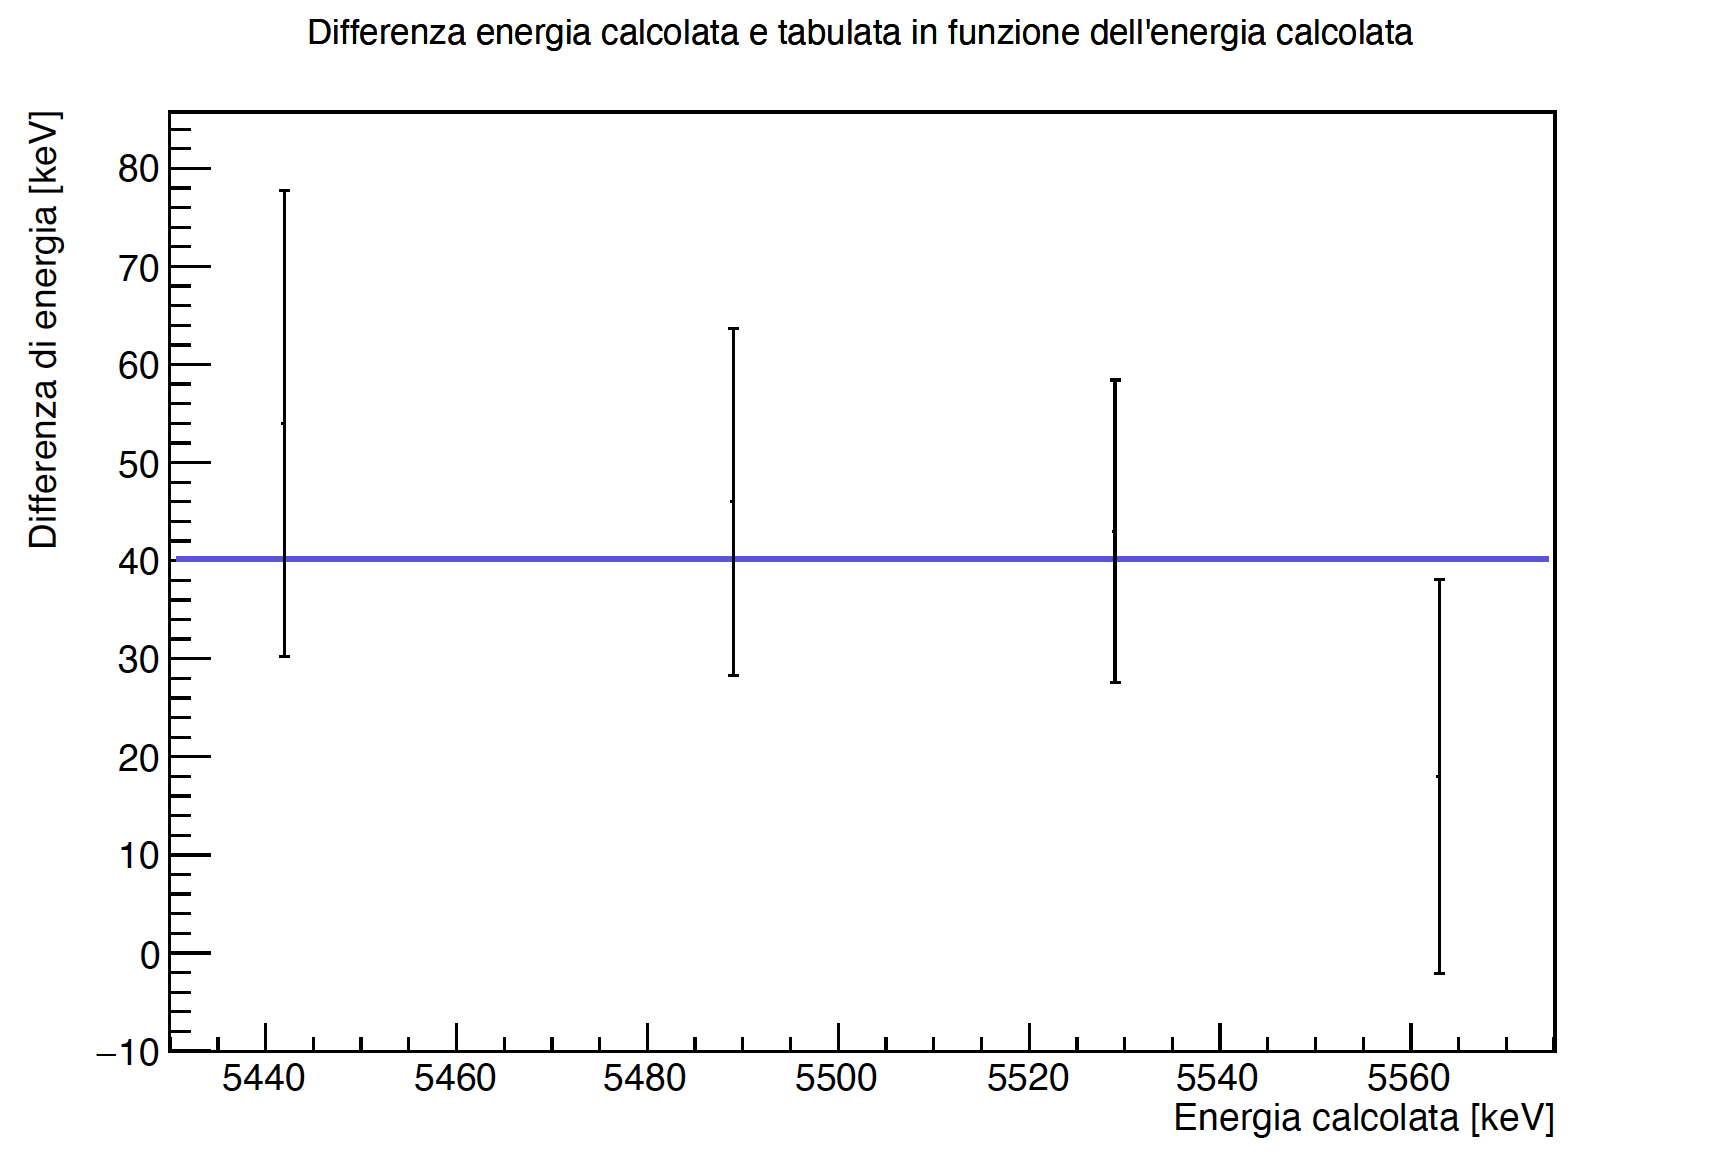
\includegraphics[scale=0.4]{discrepanza.png}
    \caption{Differenza tra energia calcolata e tabulata in funzione dell'energia calcolata}
\end{figure}

$$
    \Delta E = 40.18 \pm 9.27\, keV
$$

\noindent Analizzando le due rette di calibrazione (Figura 1 e Figura 3), quella ottenuta nella prima parte attraverso l'impulsatore e quella ottenuta dallo studio dello spettro del 241-Am, non risultano compatibili: questo \`e evidenziato dalla non compatibilit\`a dei valori di energia tabulati corrispondenti ai picchi con quelli estrapolati dalla retta di calibrazione dell'impulsatore. Questo mostra come la calibrazione ottenuta con l'impulsatore, seppur importante per evidenziare la relazione lineare fra energia e tensione, non \`e molto precisa. La calibrazione con l'americio pu\`o essere in questo senso pi\`u attendibile. Questa incongruenza pu\`o essere legata a diversi fattori: innanzitutto il 241-Am ha solo 4 picchi, per altro molto vicini, e quindi difficilmente distinguibili. Infatti, come indicato, la risoluzione dell'apparato utilizzato \`e di circa 30/40 mV e ci\`o pu\`o influenzare la forma dello spettro.\\
L'andamento della risoluzione ottenuto \`e consistente con quanto atteso per i primi 3 picchi: la risoluzione diminuisce all'aumentare dell'energia. Il fatto che il quarto ed ultimo punto non rispetti l'andamento pu\`o essere spiegato osservando lo spettro del 241-Am: l'ultimo picco, in corrispondeza del canale 4062, \`e quasi interamente coperto dal picco precendete, che corrisponde al decadimento dell'americio con il branching ratio pi\`u alto; questo rende difficile l'individuazione del picco stesso e della FWHM associata. 
\end{document} 